\documentclass[aspectratio=43,hyperref={pdfpagelabels=false}]{beamer}	 	
\usepackage{lmodern}
\usepackage{abnt-alf}
\usepackage[brazil]{babel}
\usepackage{graphicx} \graphicspath{ {../img/} } % Inclusão de gráficos
\usepackage[utf8]{inputenc}		% Codificacao do documento (conversão automática dos acentos)
\usepackage{multicol}
\usepackage{subfigure}

\usetheme{Berlin}
\usecolortheme{beaver}
\usefonttheme[onlymath]{serif}			% para fontes matemáticas
\definecolor{wine}{HTML}{8F0000}
\newcommand*\oldmacro{}%
\let\oldmacro\insertshorttitle%
\renewcommand*\insertshorttitle{%
  \oldmacro\hfill%
  \insertframenumber\,/\,\inserttotalframenumber}

\title[zorandir@gmail.com]{Aperfeiçoando a Representação de Autômatos Celulares Através de \textit{Templates}}  
\author[ ]{Zorandir Soares Jr. \\zorandir@gmail.com} 
\institute[ ]{Universidade Presbiteriana Mackenzie\\
Programa de Pós-Graduação em Engenharia Elétrica e Computação \vskip 0.5cm
Orientador: Prof. Dr. Pedro Paulo Balbi de Oliveira
}
\date{\today} 

\begin{document}

\begin{frame}
    \titlepage
\end{frame}

\begin{frame}
% \begin{multicols}{2}
    \frametitle{Sumário}
    \tableofcontents
%\end{multicols}
\end{frame}




 
 \section[Objetivos]{Objetivos e Motivação}
 \subsection*{Objetivos e Motivação}
 \begin{frame}
     \frametitle{Objetivos e Motivação}
     \begin{itemize}
           \item Aperfeiçoar a representação de autômatos celulares através de \textit{templates}
           \item Desenvolver e melhorar algoritmos geradores de templates
           \item Apresentar exemplos da utilização dos templates em problemas típicos dos ACs
           \item Pesquisar e implementar soluções para os principais problemas em aberto
     \end{itemize}
 \end{frame}
 
 




 \section{Autômatos Celulares}
 \subsection*{Autômatos Celulares}
 \begin{frame}
    \frametitle{Autômatos Celulares}

    \begin{figure}[h!]
        \centering
        
\includegraphics[width=0.6\textwidth]{fig_carpet.jpg}
        \caption{Tapetes expostos em uma exposição de arte realizada na ``Maison Salvan'', em Carjac, França, em junho de 2008. Eles foram criados com o simulador FiatLux CA.}
    \end{figure}

     % Autômatos Celulares (ACs) são idealizações matemáticas simples dos sistemas naturais. Eles consistem em um reticulado de campos discretos idênticos, onde cada campo pode assumir um conjunto finitos de, geralmente, valores inteiros. Os valores dos campos evoluem em tempo discreto de acordo com regras determinísticas que especificam o valor de cada campo de acordo com os campos das vizinhanças \cite{wolfram1994cellular}.
 \end{frame}





\begin{frame}
\frametitle{Famílias de autômatos celulares}
Uma família (ou espaço) de autômatos celulares é definida pelo raio $r$ e pelo número de estados $k$.

O tamanho de uma família é definido pela expressão abaixo:
\begin{equation}
k^{k^{2r+1}}
\label{eq:tamFamilia}
\end{equation}
\end{frame}

 \begin{frame}
     \frametitle{Propriedades Estáticas}
     \begin{itemize}
           \item Confinamento
           \item Simetria Interna Máxima
           \item Simetria Interna Arbitrária
           \item Totalidade e Semi-totalidade
           \item Conservabilidade da soma de estados
           \item Conservabilidade da soma modular de estados %(ou conservabilidade modular) %?
     \end{itemize}
 \end{frame}

% \begin{frame}
% \frametitle{Tamanho das famílias dos autômatos celulares}
% \framesubtitle{Autômatos celulares binários}
% \begin{figure}[h!]
% \centering
% 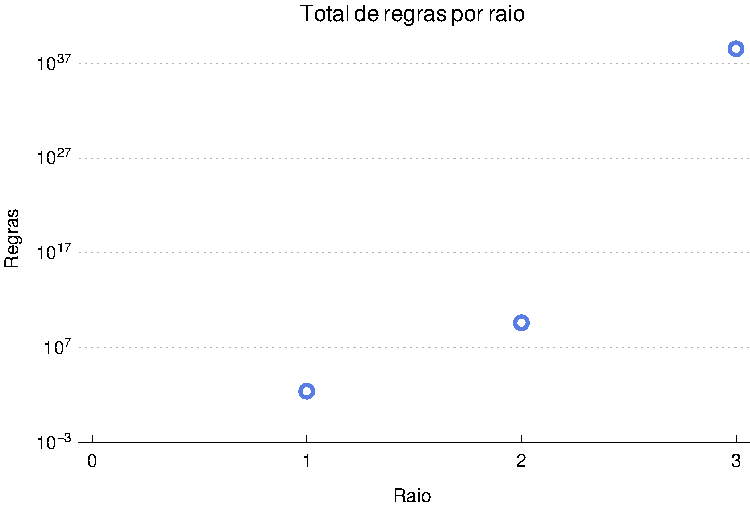
\includegraphics[width=.5\textwidth]{fig_graphicRxr.pdf}
% \caption{Gráfico mostrando a variação do tamanho dos espaços de acordo com o tamanho do raio $r$}
% \end{figure}
% \end{frame}

% \begin{frame} %Substitiur por um BOM gráfico
% \frametitle{Tamanho das famílias dos autômatos celulares}
% \framesubtitle{Autômatos celulares não binários}
% \begin{figure}[h!]
% \centering
% 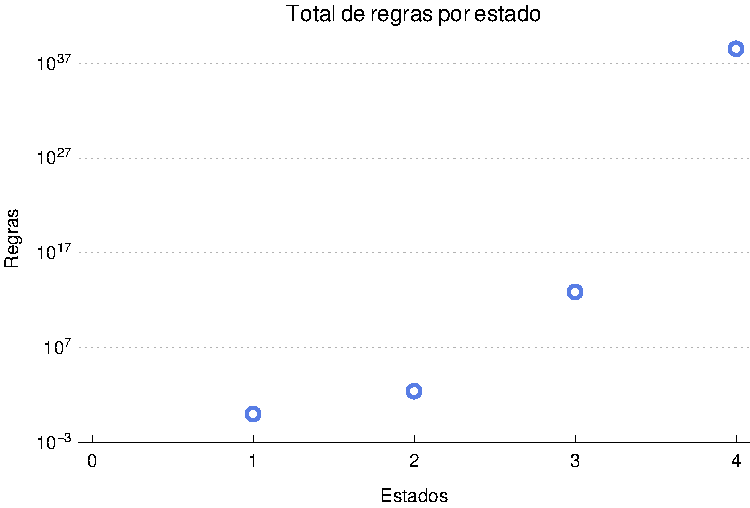
\includegraphics[width=.5\textwidth]{fig_graphicRxk.pdf}
% \caption{Gráfico mostrando a variação do tamanho dos espaços de acordo com o número de estados $k$}
% \end{figure}
% \end{frame}

%  \begin{frame}
%      \frametitle{Representação de famílias}
%      \framesubtitle{Grafos de Gruijin}
%  \end{frame}

% \begin{frame}
% 	\frametitle{Representação de famílias}
% 	\framesubtitle{Templates}
% \end{frame}






\section{Templates}
\subsection*{Templates}
\begin{frame}
	\frametitle{Templates}
	
	\textit{Template} é uma generalização de tabelas de transições de ACs.
    \begin{figure}[h!]
        \centering
        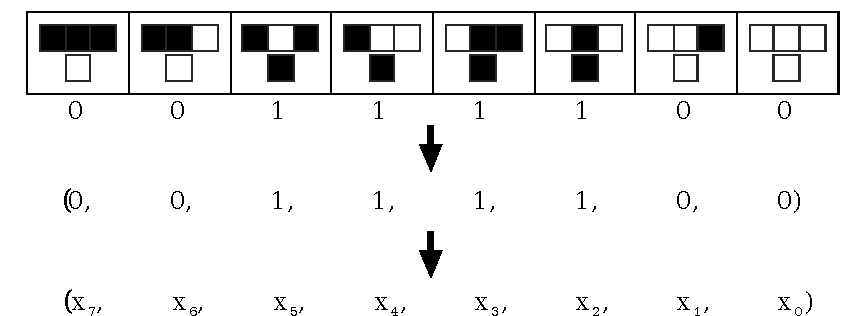
\includegraphics[width=0.6\textwidth]{fig_transitionTable.pdf}
        \caption{Exemplo de tabelas de transições}
    \end{figure}
\end{frame}

\begin{frame}
    \frametitle{Exemplo -  Template Base}
    
    \begin{equation}
    \begin{split}
    (k:2, r:1, \\rawList:(x_7,x_6,x_5,x_4,x_3,x_2,x_1,x_0),  \\expansionFunction:RawExpansion)
    \end{split}
    \end{equation}
\end{frame}

\begin{frame}
    \frametitle{Exemplo -  Template Modular}
  
    \begin{equation}
    \begin{split}
    (k:2, r:1, N:2, \\rawList:(x_7,x_6,x_5,x_4,x_3,x_2,x_1,x_0),  \\imprisonmentExpressions:(x_0 \in \{0,1\}), \\expansionFunction:ModNExpansion)
    \end{split}
    \end{equation}
\end{frame}

\begin{frame}
	\frametitle{Expansão}
	Expansão é o processo no qual se obtêm todas as tabelas de transição $R_k$ associadas a um template $T$.
    \begin{columns}
    \begin{column}{5cm}
        \begin{equation}
        E(T)=R_k
        \end{equation}
    \end{column}
    \pause
    \begin{column}{5cm}
     \begin{itemize}
           \item RawExpansion
           \item FilteredExpansion
           \item ModNExpansion
     \end{itemize}
    \end{column}
    \end{columns}
 \end{frame}

\begin{frame}
	\frametitle{Intersecção}
	\begin{equation}
	I(T_1,T_2)=T_3 \Leftrightarrow E(T_3) = E(T_1) \cap E(T_2)
	\end{equation}

    \begin{figure}[h!]
      \centering
      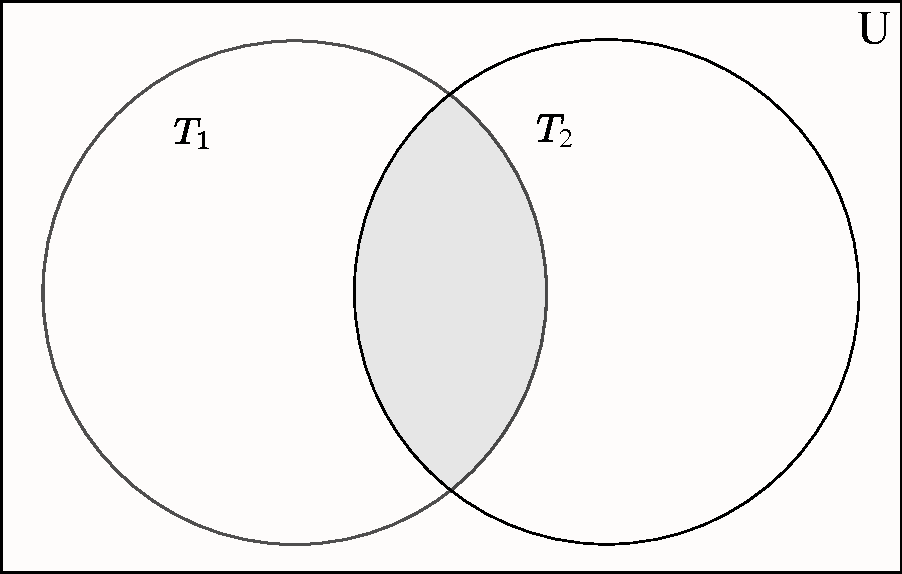
\includegraphics[width=.4\textwidth]{fig_intersection.pdf}
      \caption{Os círculos $T_1$ e $T_2$ são templates que representam dois conjuntos de regras. Em cinza, $T_3$ é o template que representa o conjunto de regras de intersecção entre $T_1$ e $T_2$.}
      \label{fig:intersection}
    \end{figure}        
    % Intersecção é o processo no qual se obtêm um template que represente o conjunto $R_k$ após se receber dois templates definidos para o mesmo espaço. A operação de intersecção também foi implementada por \cite{daCosta2014} e foi descrita em maior detalhes da seguinte maneira:

 \end{frame}

 \begin{frame}
    \frametitle{Intersecção}

    \textbf{Intersecções resolvidas}
    \begin{itemize}
      \item Intersecção de templates não modulares
      \item Intersecção de templates modulares com mesmo valor de $N$
    \end{itemize}
 \end{frame}

\begin{frame}
    \frametitle{Complemento}
    \begin{equation}
    C(T_1)=\bar{T}_1 \Leftrightarrow E(\bar{T}_1) = U \setminus E(T_1)
    \end{equation}

    \begin{figure}[h!]
      \centering
      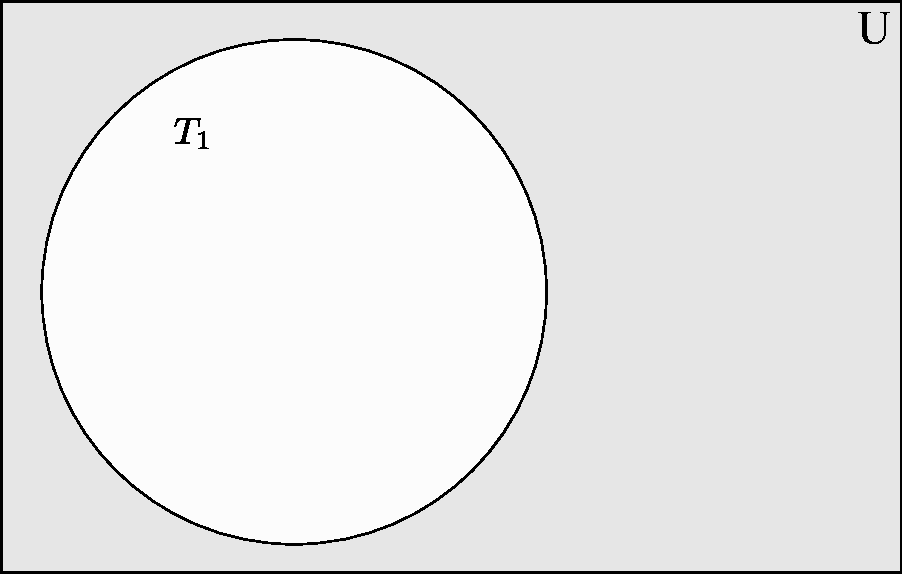
\includegraphics[width=.4\textwidth]{fig_complement3.pdf}
      \caption{Em branco, $T_1$ é um template que representa um conjunto de regras. Em cinza, $\bar{T_1}$ é um conjunto de template que representa o complemento de $T_1$.}
      \label{fig:complement}
    \end{figure}    
 \end{frame}

% \begin{frame}
%     \frametitle{Confinamento}
%     \framesubtitle{Operação Geradora de Templates}
%           \vspace{-0.8cm}
%     \begin{itemize}
%            \item Implementado na CATemplates
%            \item Funciona com qualquer número de estados
%      \end{itemize}     
%         \begin{equation}
%         \begin{split}
%         (k:2, r:1, \\rawList:(1, x_6, x_5, x_4, x_3, x_2, x_1, 0),  \\expansionFunction:RawExpansion)
%         \end{split}
%         \end{equation}        
% \end{frame}

% \begin{frame}
%     \frametitle{Totalidade e Semi-Totalidade}
%     \framesubtitle{Operação Geradora de Templates}
%           \vspace{-0.8cm}
%     \begin{itemize}
%            \item Implementado na CATemplates
%            \item Funciona com qualquer número de estados
%      \end{itemize}     
%     \begin{equation}
%     \begin{split}
%     (k:2, r:1, rawList:(x_7, x_3, x_3, x_1, x_3, x_1, x_1, 0),  \\expansionFunction:RawExpansion)
%     \end{split}
%     \end{equation}        
%     \begin{equation}
%     \begin{split}
%     (k:2, r:1, rawList:(x_7, x_3, x_5, x_1, x_3, x_2, x_1, 0),  \\expansionFunction:RawExpansion)
%     \end{split}
%     \end{equation}    
% \end{frame}

% \begin{frame}
%     \frametitle{Color Blind}
%     \framesubtitle{Operação Geradora de Templates}
%      \vspace{-0.8cm}
%      \begin{itemize}
%            \item Implementado na CATemplates
%            \item Funciona com qualquer número de estados
%            \item Template Modular para $k>2$
%      \end{itemize}     
%         \begin{equation}
%         \begin{split}
%         (k:3, r:1, rawList:(2, 2 - x_1, 2 - 2 x_1, 2 - x_3, 2 - x_4, 2 - x_5, 2 - 2 x_3,\\
%          2 - 2 x_5, 2 - 2 x_4, 1 - 2 x_4, 1 - 2 x_3, 1 - 2 x_5, 1 - 2 x_1, 1, 1 + 2 x_1, 1 + 2 x_5,\\
%                       1 + 2 x_3, 1 + 2 x_4, 2 x_4, 2 x_5, 2 x_3,x_5, x_4, x_3, 2 x_1, x_1, 0), \\expansionFunction:ModKExpansion)
%         \end{split}
%         \end{equation}    
% \end{frame}

% \begin{frame}
%     \frametitle{Simetria Interna Máxima}
%     \framesubtitle{Operação Geradora de Templates}
%      \vspace{-0.8cm}
%      \begin{itemize}
%            \item Implementado no CATemplates
%            \item Funciona com qualquer número de estados
%      \end{itemize}     
%         \begin{equation}
%         \begin{split}
%         rawList:(x_7, x_3, x_5, x_1, x_3, x_2, x_1, x_0)
%         \end{split}
%         \end{equation}        
%         \begin{equation}
%         \begin{split}
%         rawList:(1 - x_0, 1 - x_1, 1 - x_2, 1 - x_3, x_3, x_2, x_1, x_0)
%         \end{split}
%         \end{equation}
%         \begin{equation}
%         \begin{split}
%         rawList:(1 - x_0, 1 - x_4, 1 - x_2, 1 - x_4, x_3, x_2, x_1, x_0)
%         \end{split}
%         \end{equation}   
% \end{frame} 

% \begin{frame}
%     \frametitle{Simetria Interna Arbitrária}
%     \framesubtitle{Operação Geradora de Templates}
%      \vspace{-0.8cm}
%      \begin{itemize}
%            \item Implementado na CATemplates
%            \item Funciona apenas no espaço binário
%      \end{itemize}     
%         \begin{equation}
%         \begin{split}
%         (k:2, r:1, \\rawList:(x_7, x_3, x_3, x_1, x_3, x_1, x_1, 0),  \\expansionFunction:RawExpansion)
%         \end{split}
%         \end{equation}        

% \end{frame} 

% \begin{frame}
%     \frametitle{Conservabilidade de Estados}
%     \framesubtitle{Operação Geradora de Templates}
%      \vspace{-0.8cm}
%      \begin{itemize}
%            \item Implementado na CATemplates
%            \item Funciona com qualquer número de estados
%      \end{itemize}     
%         \begin{equation}
%         \begin{split}
%         (k:2, r:1, \\rawList:(1, 1 + x_2 - x_3, 1 - x_2, 1 - x_1 - x_2, x_3, x_2, x_1, 0),  \\expansionFunction:RawExpansion)
%         \end{split}
%         \end{equation}        
% \end{frame} 

% \begin{frame}
%     \frametitle{Conservabilidade Modular}
%     \framesubtitle{Operação Geradora de Templates}
%      \vspace{-0.8cm}
%      \begin{itemize}
%            \item Implementado na CATemplates
%            \item Funciona com qualquer número de estados
%            \item Template Modular
%      \end{itemize}     
%         \begin{equation}
%         \begin{split}
%         (k:2, r:1, n:2, \\rawList:(1, 1 + x_2 + x_3, 1 + x_2, 1 + x_1 + x_2, x_3, x_2, x_1, 0),  \\expansionFunction:ModNExpansion)
%         \end{split}
%         \end{equation}        
% \end{frame} 

\begin{frame}
    \frametitle{Geradoras de Templates e Número de Estados}
    \vspace{-0.8cm}
    \begin{table}[]
    \centering
    \caption{Compatibilidade entre algoritmos geradores de templates e número de estados }
    \vspace{-0.8cm}
    \label{my-label}
    \resizebox{\textwidth}{!}{
    \vspace{0cm}
    \begin{tabular}{|l|l|l|}
    \hline
                                               & \multicolumn{2}{c|}{Número de Estados} \\ \hline
    \textbf{Algoritmos Geradores de Templates} & $k=2$                              & $k\textgreater2$                          \\ \hline
    Totalidade e Semi-Totalidade               &  •                                 & •                                         \\ \hline
    Confinamento                               &  •                                 & •                                         \\ \hline
    Color Blind                                &  •                                 & •\footnote{Template Modular}              \\ \hline
    Simetria Máxima                            &  •                                 & •                                         \\ \hline
    Simetria Arbitrária                        &  •                                 &                                           \\ \hline
    Conservabilidade da soma de estados                &  •                                 & •                                         \\ \hline
    Conservabilidade da soma modular de estados                &  •\footnotemark[\value{footnote}]  &                                           \\ \hline
    \hline
    \end{tabular}
    }
\end{table}
\end{frame} 



 \section{Resultados Parciais}
 \subsection*{Resultados Parciais}
 \begin{frame}
     \frametitle{Resultados Parciais}
     \begin{itemize}
           \item Aplicação no Problema de Paridade
           \item Operação de Complemento
     \end{itemize}
 \end{frame}

\begin{frame}
    \frametitle{Problema de Paridade}
    \begin{figure}[h!]
        \centering
        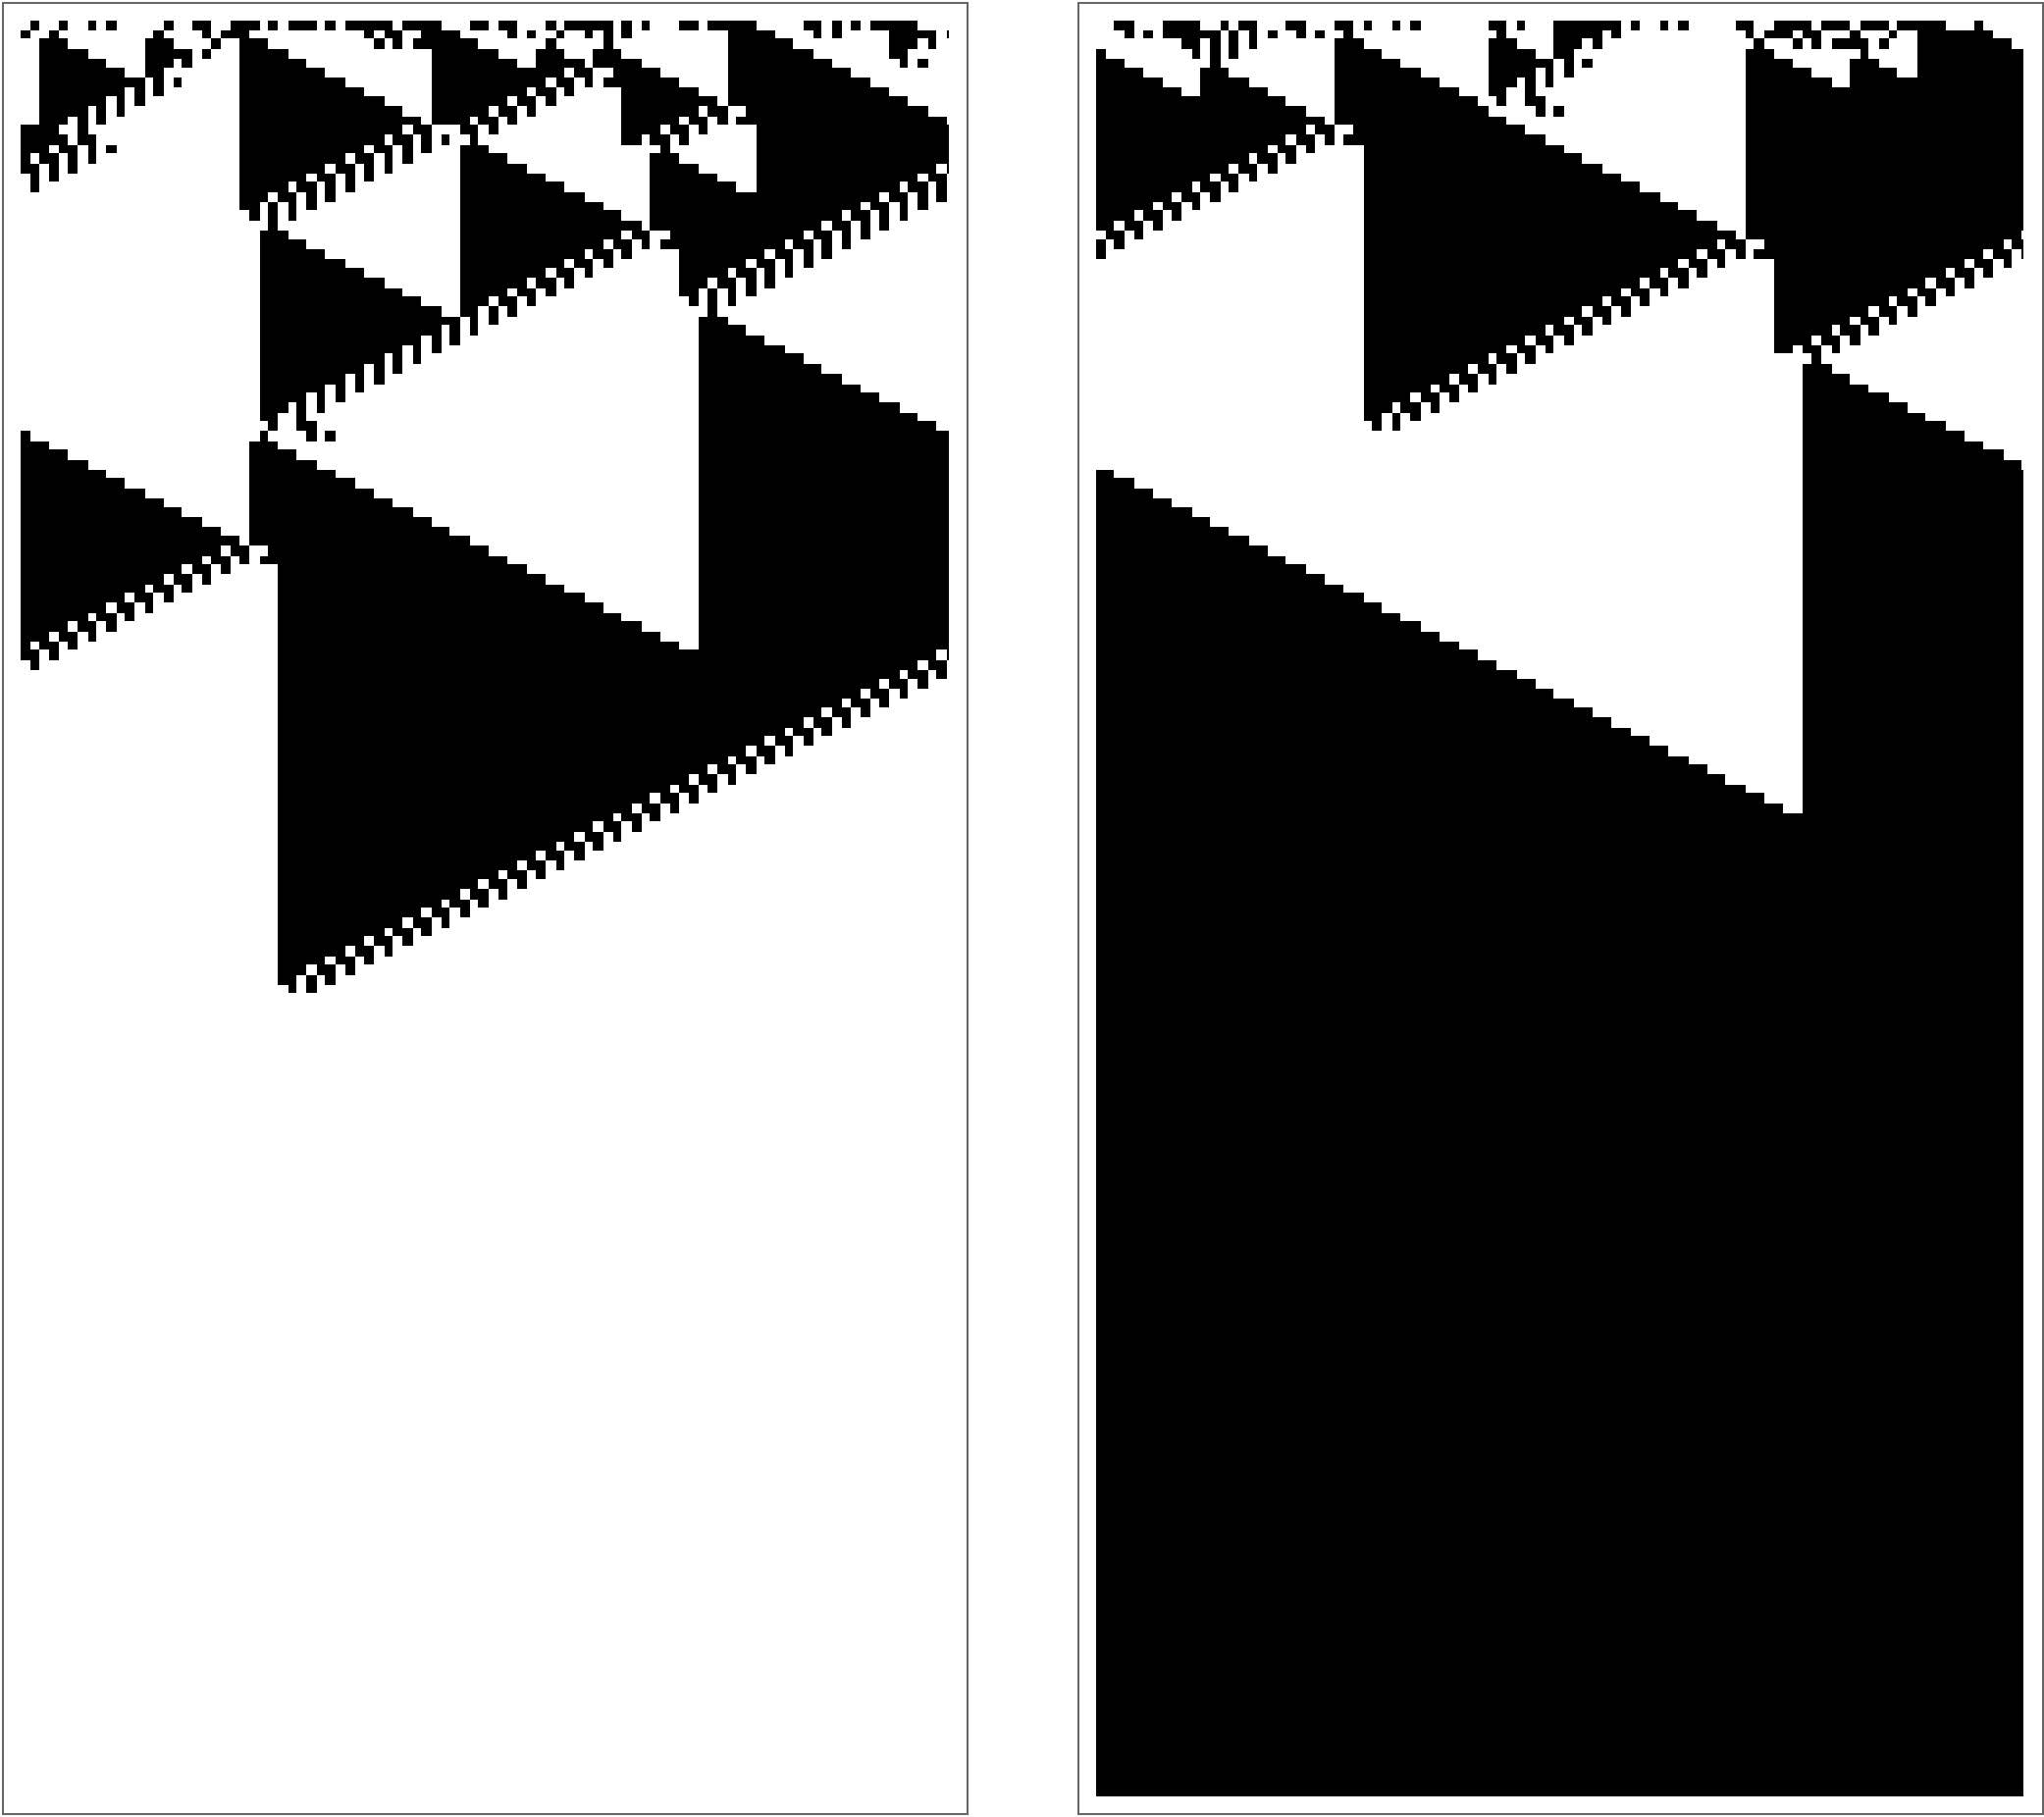
\includegraphics[width=0.5\textwidth]{fig_parityRule.pdf}
        \caption{Exemplo de regra de paridade. A imagem a esquerda contém em sua entrada um número par de 1s. A da direita contém um número ímpar.}
    \end{figure}
\end{frame}

\begin{frame}
    \frametitle{Problema de Paridade}
    \begin{equation}
    T_{paridade} = (T_{conservaparidade} \cap T_{confinado}) \cap \bar{T}_{conservaestados}
    % T_{paridade} = T_{conservaparidade} \cap \bar{T}_{conservaestados}
    \label{eq:operationsTemplateParidade}
    \end{equation}

    \begin{alertblock}{A regra que solucione o problema de paridade:}
        \vspace{-0.4cm}    
        \begin{itemize}
          \item deve ser \textbf{confinada}
          \item deve \textbf{conservar a paridade}
          \item não deve \textbf{number conserving}
        \end{itemize}
    \end{alertblock}
\end{frame}

\begin{frame}
    \frametitle{Problema de Paridade}

    Tamanho do espaço:
    \begin{equation}
    2^{2^{2\times3+1}}=3,4 \times 10^{38}
    \end{equation}

    Número máximo de regras conservativas de paridade:
    \begin{equation}
    2^{63} \approx  9.2\times 10^{18}
    \end{equation}

    


\end{frame}

\begin{frame}
    \frametitle{Complemento}
    \begin{columns}
        \begin{column}{5cm}
    \begin{equation}
    rawList:(x_7, x_6, x_5, 1 - x_1, x_3, x_2, x_1, 0)
    \end{equation}
    \begin{equation}
    \left\{\begin{matrix}
    x_7 & = & x_7   \\ 
    x_6 & = & x_6   \\ 
    x_5 & = & x_5   \\ 
    x_4 & = & 1 - x_1 \\ 
    x_3 & = & x_3   \\ 
    x_2 & = & x_2   \\ 
    x_1 & = & x_1   \\ 
    x_0 & = & 0
    \end{matrix}\right.
    \end{equation}
    \begin{equation}
    x_4 = 1 - x_1 \wedge x_0 = 0
    \end{equation}
    \end{column}

    \begin{column}{5cm}
        \begin{figure}[h!]
          \centering
          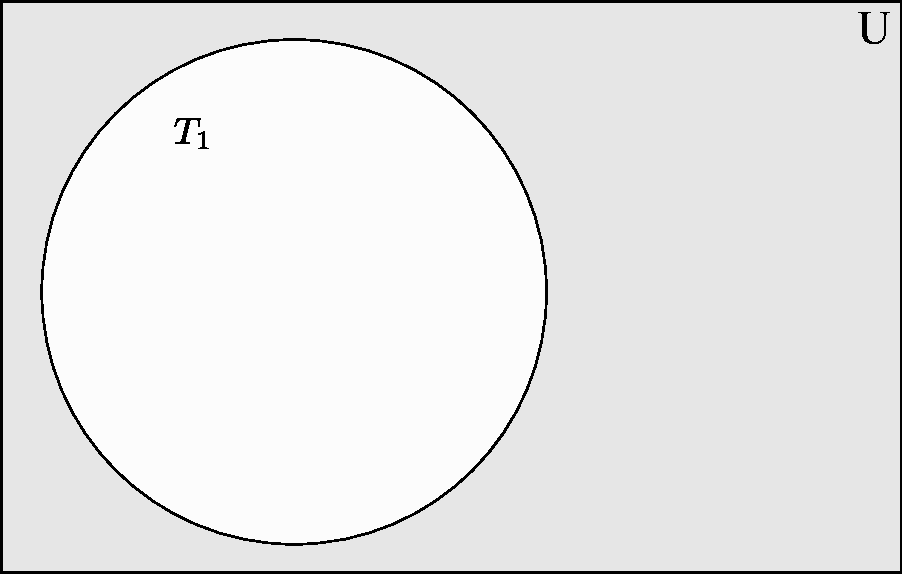
\includegraphics[width=.8\textwidth]{fig_complement3.pdf}
        \end{figure}
    \end{column}
\end{columns}
\end{frame}

\begin{frame}
    \frametitle{Complemento}
    \begin{columns}
        \begin{column}{5cm}
        \begin{equation}
        x_4 = 1 - x_1 \vee x_0 = 0
        \end{equation}
        \begin{equation}
        x_4 = 1 - (1 - x_1) \vee 
        x_0 = 1 - 0
        \end{equation}
        \begin{equation}
        S = \{\{x_4 \to x_1\},\{x_0\to 1\}\}
        \end{equation}
    \end{column}

    \begin{column}{5cm}
        \begin{figure}[h!]
          \centering
          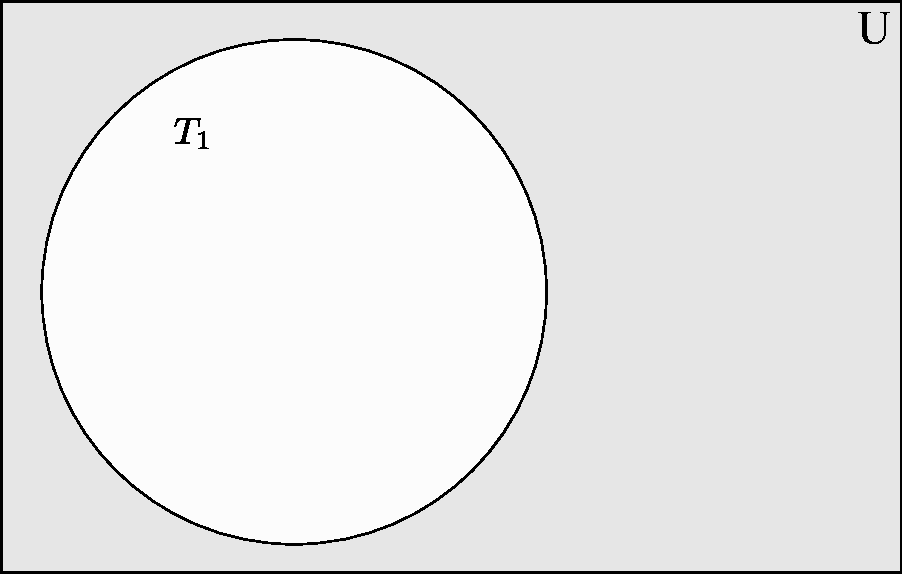
\includegraphics[width=.7\textwidth]{fig_complement3.pdf}
        \end{figure}
    \end{column}
\end{columns}
\begin{equation}
\{(x_7, x_6, x_5, x_4, x_3, x_2, x_1, 1),(x_7, x_6, x_5, x_1, x_3, x_2, x_1, x_0)\}
\end{equation}
\end{frame}

% \begin{frame}
%     \frametitle{Problema de Paridade}
%     \framesubtitle{Aplicação}
   
%     O \textit{Problema de Paridade}. Neste problema a configuração inicial (entrada) deve ser classificada em uma entre duas classe, de acordo com a quantidade par de 1s ou não (a saída é, portanto, a paridade da entrada - par ou ímpar) \cite{Sipper1998}.
% \end{frame}






 \section{Problemas e Trabalhos Futuros}
 \subsection*{Problemas em Aberto}
 \begin{frame}
    \frametitle{Intersecção de Templates Modulares}

    \textbf{Intersecções não resolvidas}
    \begin{itemize}
      \item Intersecção de templates com Mods diferentes
      \item Intersecção de um template modular com um template não modular
    \end{itemize}

    \begin{alertblock}{Solução do problema permite:}
        \vspace{-0.4cm}
        \begin{itemize}
          \item Realizar o complemento de Templates Modulares 
          \item Criar a operação de diferença entre Templates
        \end{itemize}
    \end{alertblock}
 \end{frame}


\begin{frame}
    \frametitle{Intersecção de Templates Modulares primos entre si}
    \begin{alertblock}{Teorema Chinês dos restos}
    \vspace{-0.4cm}    
    \label{chinese}
    Sejam $m_1,m_2,\dots,m_r$, $r$ inteiros positivos que são primos entre si, dois a dois, e sejam $a_1,a_2,\dots,a_r$, $r$ inteiros quaisquer. Então, o sistema de congruências:
    
    $
        \left\{\begin{matrix}
        x \equiv a_1 & (\textup{mod }m_1) \\ 
        x \equiv a_2 & (\textup{mod }m_2) \\
        \vdots \\
        x \equiv a_r & (\textup{mod }m_r) \\
        \end{matrix}\right.    
    $

    admite um solução $x$ única módulo $m = m_1 m_2 \dots m_r$
    \end{alertblock}
\end{frame} 

 \begin{frame}
     \frametitle{Negação de variável}
     No caso binário, uma variável pode ser negada por meio da função $f(x)=1-x$. No template abaixo a terceira posição ilustra a variável $x_1$ negada. 
    \begin{equation}
    \begin{split}
    (k=2, r=0.5, \\
    rawList= (1,1-x_1,x_1,0), \\
    expansionFunction=RawExpansion)
    \end{split}
    \end{equation}
 \end{frame}

 \begin{frame}
     \frametitle{Negação de variável}
     A questão: como negar variáveis em templates não binários?

    \begin{alertblock}{Solução do problema permite:}
        \vspace{-0.4cm}
        \begin{itemize}
          \item Abstração do algoritmo gerador de templates de simetria interna.
          \item Abstração da operação de complemento.
        \end{itemize}
    \end{alertblock}
 \end{frame}

  \begin{frame}
    \frametitle{Operação de Diferença entre Conjuntos}
    \begin{equation}
    C(T_1,T_2)=T_3 \Leftrightarrow E(T_3) = E(T_2) \setminus E(T_1)
    \end{equation}

    \begin{figure}[h!]
      \centering
      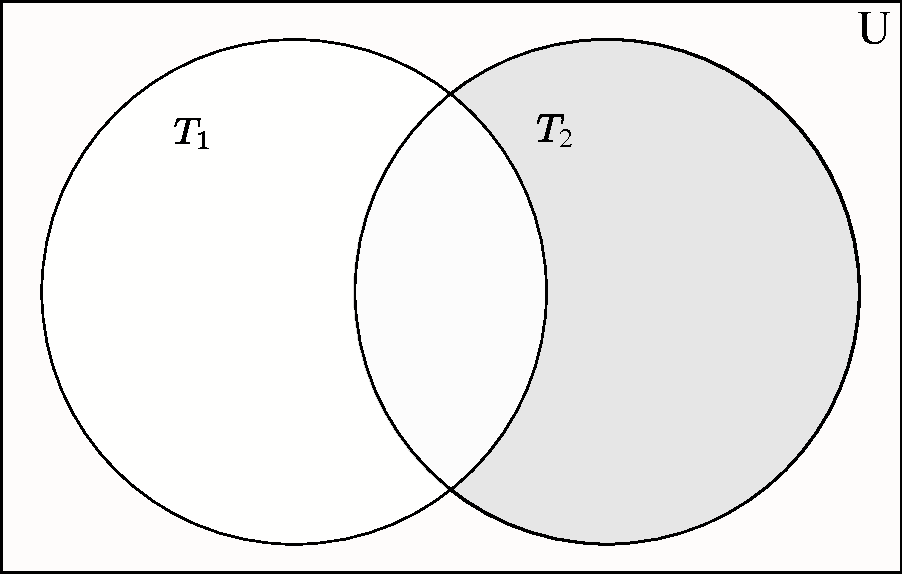
\includegraphics[width=.4\textwidth]{fig_complement2.pdf}
      \caption{Os círculos $T_1$ e $T_2$ são os templates que representam dois conjuntos de regras. Em cinza, $T_3$ é um conjunto de template que representa o conjunto de regras de $T_2 - T_1$.}
      \label{fig:complement2}
    \end{figure}    
 \end{frame}

 \section{Cronograma}
 \subsection*{Cronograma}

 \begin{frame}
     \frametitle{Cronograma}
      \begin{itemize}
          \item Fase 0: participação nas disciplinas necessárias ao cumprimento dos créditos para a obtenção do título de mestre;
          \item Fase 1: pesquisa bibliográfica de autômatos celulares e de templates;
          \item Fase 2: programação e testes da operação de complemento de templates;
          \item Fase 3: proposição de propriedades estáticas para se gerar templates;
          \item Fase 4: pesquisa e implementação dos problemas em abertos e de novas operações de geração de templates;
          \item Fase 5: submissão de artigo;
          \item Fase 6: escrita da dissertação.
      \end{itemize}
 \end{frame}

 \begin{frame}
     \frametitle{Cronograma}
\begin{table}[h!]
\centering
\caption{Cronograma de desenvolvimento do projeto}
\vspace{-0.8cm}
\label{cronograma}
\resizebox{\textwidth}{!}{
    \vspace{0cm}
    \begin{tabular}{|l|c|c|c|c|c|c|c|c|}
    \hline  
    \multicolumn{1}{|c|}{}  & \multicolumn{4}{c|}{2014}                     & \multicolumn{4}{c|}{2015}                     \\ \hline
    \textbf{Atividades}     & Jan-Mar   & Abr-Jun   & Jul-Set   & Out-Dez   & Jan-Mar   & Abr-Jun   & Jul-Set   & Out-Dez   \\ \hline
    Fase 0                  &  •        & •         & •         & •         &           & •         &           &           \\ \hline
    Fase 1                  &           &           &           & •         &  •        &           &           &           \\ \hline
    Fase 2                  &           &           &           &           &  •        & •         &           &           \\ \hline
    Fase 3                  &           &           &           &           &           &           & •         &           \\ \hline
    Fase 4                  &           &           &           &           &           &           & •         & •         \\ \hline
    Fase 5                  &           &           &           &           &           &           & •         &           \\ \hline
    Fase 6                  &           &           &           &           &           & •         & •         & •         \\ \hline
    \hline
    \end{tabular}
}
\end{table}
 \end{frame}





% \section{Referências}
%  \begin{frame}%[allowframebreaks]
%      \frametitle{Referências}
%      \bibliography{bibliografia}
%  \end{frame}





 % \section{}
 % \begin{frame}[t]\frametitle{Dúvidas}
 %     \center
 %     {\fontsize{250}{300}\selectfont {?}}
 % \end{frame}




\section*{}
\begin{frame}[t]
     \frametitle{Agradecimentos}
\vspace{1cm}
\center
     À Capes, CNPq, MackPesquisa e ao Laboratório de Computação Natural (LCoN).

    % \center
    % {\fontsize{50}{300}\selectfont {Obrigado}}
\end{frame}
\end{document}
